% -*- TeX-master: "main"; fill-column: 72 -*-

\section{Package syntax and semantics}
\label{sec:syntax}

In this section, we define the syntax and semantics of the Hierarchical
Model Composition package for SBML Level~3 Version~1.  We expound on the
various data types and constructs defined in this package, then in
\sect{examples}, we provide complete examples of using the constructs in
example SBML models.


% -----------------------------------------------------------------------------
\subsection{Primitive data types}
\label{new-primitive-types}

Section~3.1 of the SBML Level~3 specification defines a number of
primitive data types and also uses a number of XML Schema 1.0 data
types~\citep{biron:2000}.  We assume and use some of them in the rest of
this specification, specifically \primtype{boolean}, \primtype{ID},
\primtype{IDREF}, \primtype{SId}, \primtype{SIdRef}, \primtype{UnitSId},
\primtype{UnitSIdRef}, and \primtype{string}.  The Hierarchical Model
Composition package also makes use of or defines other primitive types;
they are described below.


\subsubsection{Type \hspace*{1pt}\primtypeNC{anyURI}}
\label{primtype-anyuri}
\label{primtype-uri}

Type \primtype{anyURI} is defined by XML Schema 1.0.  It is a character
string data type whose values are interpretable as URIs (\emph{Universal
  Resource Identifiers}; \citealt{harold:2001,w3c:2000}) as described by
the W3C document RFC~3986~\citep{rfc3986}.


\subsubsection{Type \hspace*{1pt}\primtypeNC{PortSId}}
\label{primtype-portid}

The type \primtype{PortSId} is derived from \primtype{SId} (SBML Level~3
Version~1 Core specification Section~3.1.7) and has identical syntax.
The \primtype{PortSId} type is used as the data type for the identifiers
of ports (Section~\ref{port-class}) in the Hierarchical Model Composition
package.  The purpose of having a separate type for such identifiers is
to enable the space of possible port identifier values to be separated
from the space of all other identifier values in SBML.  The equality of
\primtype{PortSId} values is determined by an exact character sequence
match; i.e., comparisons of these identifiers must be performed in a
case-sensitive manner.


\subsubsection{Type \hspace*{1pt}\primtypeNC{PortSIdRef}}
\label{primtype-portidref}

Type \primtype{PortSIdRef} is used for all attributes that refer to
identifiers of type \primtype{PortSId}.  This type is derived from
\primtype{PortSId}, but with the restriction that the value of an
attribute having type \primtype{PortSIdRef} must match the value of a
\primtype{PortSId} attribute in the relevant model;  in other words, the value of
the attribute must be an existing port identifier in
the referenced model.  As with \primtype{PortSId}, the equality of
\primtype{PortSIdRef} values is determined by exact character sequence
match; i.e., comparisons of these identifiers must be performed in a
case-sensitive manner.


% -----------------------------------------------------------------------------
\subsection{Namespace scoping rules for identifiers}
\label{namespaces}

In the Hierarchical Model Composition package, as in SBML Level~3
Version~1 Core, the \Model object contains the main components of an
SBML model, such as the species, compartments and reactions.  The package adds the
ability to put \emph{multiple} models inside an SBML document, and therefore must define the scope of
identifiers in such a way that identifier collisions are prevented.

Although the definitions of the main constructs in the package are not
presented until later in this section, the scoping rules apply to all
constructs and therefore are appropriate to discuss separately.  Here
are the rules:

\begin{enumerate}

\item A shared namespace exists for \primtype{SId} values defined at the
  SBML document level.  This namespace applies to the identifiers of
  \Model and \ExternalModelDefinition objects within the SBML document.
  The identifier of every \Model and \ExternalModelDefinition object
  must be unique across the set of all such identifiers in the document.
  The namespace is limited to that SBML document, and is not shared with
  any other SBML document, even if that document is referenced via an
  \ExternalModelDefinition.  This namespace is known as \emph{the model
    namespace of the document}.

\item The namespace for \primtype{SId} identifiers defined \emph{within}
  a \Model object used in Hierarchical Model Composition follows the
  same rules as those defined in SBML Level~3 Core for plain \Model
  objects.  That is, the scope of the identifiers is limited to the
  enclosing \Model object.  This means that two or more \Model objects
  in the same document may reuse the same identifiers---identifiers do not need to be unique
  at the level of the SBML document.  (For example, two model
  definitions could use the same \primtype{SId} value for
  \Parameter objects within their respective contents.  However, this
  does \emph{not} imply that the two objects are equated with each
  other!)  This is known as the \emph{object namespace of the model}.
  An implication of this rule is that to fully locate an object when
  there are multiple models in an SBML document, one must know not only
  the object's identifier, but also the identifier of the model in which
  it is located.

\item As in SBML Level~3 Version~1 Core, the identifier of every
  \UnitDefinition object must be unique across the set of all such
  identifiers in the \Model to which they belong.  This is referred to
  as the \emph{unit namespace of the model}.  Similar to the case above,
  an implication of this rule is that to fully locate a user-defined
  unit definition when there are multiple models in an SBML document,
  one must know not only the unit definition's identifier, but also the
  identifier of the model in which it is located.

\item The Hierarchical Model Composition package defines a new kind of
  component: the port, represented by \Port objects.  The identifier of
  every \Port object must be unique across the set of all such
  identifiers in the \Model object to which they belong.  Again, an
  implication of this rule is that to fully locate a port when there are
  multiple models in an SBML document, one must know not only the port's
  identifier, but also the identifier of the model in which it is
  located.

\item \Reaction objects introduce a local namespace for \LocalParameter
  objects.  These objects cannot be referenced from outside a given
  reaction definition.  For the Hierarchical Model Composition package,
  the implication is that the the \SBaseRef class (\sect{sbaseref-class})
  cannot reference reaction local parameters by their identifiers.
  However, the \LocalParameter objects \emph{can} be given meta
  identifiers (i.e., a value for their \SBase-derived \token{metaid}
  attribute) and be referenced using those.

% FIXME need move this somewhere else:
% 
%   If replaced, it must be by an element in the normal element namespace of
%   a model (such as a global Parameter).  Old references to that replaced
%   LocalParameter will then point to the new replacement element.  If a
%   LocalParameter is deleted from a Reaction whose KineticLaw used it in
%   its math, that KineticLaw may still be valid if there was an element
%   in the element namespace of the model with that same id to which it
%   can now refer (in other words, if the LocalParameter shadowed a global
%   parameter).


\end{enumerate}

The following example may clarify some of these rules.  Suppose a given
SBML document contains a \Model object having the identifier \val{mod1}.
This \Model cannot contain another object with the same identifier
(e.g., it could not have a \Parameter object with the identifier
\val{mod1}), nor can there be any other \Model or
\ExternalModelDefinition objects identified as \val{mod1} within the
same SBML document.  The first restriction is simply the regular SBML
rule about uniqueness of identifiers throughout a \Model object; the
second restriction is due to point (1) above.  On the other hand, there
could be a second \Model object in the same document containing a
component (e.g., a \Parameter) with the identifier \val{mod1}.  This
would not conflict with the first \Model identifier (because the
\Parameter would be effectively hidden at a lower level within the
second \Model).


% -----------------------------------------------------------------------------
\subsection{The extended \class{SBML} class}
\label{sbml-class}
\label{listofmodeldefinitions-class}
\label{listofexternalmodeldefinitions-class}

The top level of an ``SBML document'' is a container whose structure is
defined by the object class \SBML in the SBML Level~3 specification.  In
Level~3 Core, this container can contain only one model, an object of
class \Model.  As outlined in the introduction (\sect{intro}), the
purpose of the Hierarchical Model Composition package is to allow SBML
documents to contain \emph{more} than one model.  To explain how this is
accomplished, we first need to introduce some new terms to help in our
explanations.

In the approach taken here, we make a distinction between (a) the
definition of a model, before it is actually used anywhere, and (b) the
actual use of a model inside another.  We use the term \emph{model
  definition} for the former, and \emph{submodel} for the latter.  A
model definition is akin to a Platonic ideal: it may be a complete model
in and of itself, but until it is instantiated, it exists only as a
concept.  A submodel, on the other hand, is an instantiation or instance
of a previously-defined model: it is the realization of that model
inside another model.  From the perspective of the model that contains
the submodel, it has come into being, and now exists as something that
can be used (and possibly modified and adapted, as we will explain
later).  If the containing model is the \Model object of the SBML file,
it has been fully instantiated.  If the containing model is instead
another model definition, the submodel becomes part of that larger
model, but has not been fully instantiated in the SBML document until
that model definition is itself instantiated in the \Model object.

Past proposals for model composition in SBML tended to call model
definitions themselves the ``submodels''.  We avoid that term because the
model definitions must be valid \Model objects in and of themselves, and
may be used standalone (i.e., may not ever be included inside another
model).  Instead, we reserve the term ``submodel'' specifically for the
instance of a model inside a containing model.  Another term proposed in
prior work is ``model template'', which is close to what is intended by
our use of the term model definition, but tends to imply that the model
in question is somehow incomplete and needs to be filled in.  While this
is indeed possible in the scheme described here, it is not required; for
example, in a model aggregation situation, several complete working
models may be integrated to form a larger whole.  We therefore eschew
the term ``model template'' in favor of \emph{model definition}.

The components that are used to implement these notions of model
definition and submodel are defined in
Figures~\ref{hierarchical-sbml-uml}--\ref{submodel-uml} in the pages
that follow.  The extension of SBML Level~3's standard \SBML class
consists of adding two new lists, \token{listOfModelDefinitions} and
\token{listOfExternalModelDefinitions}, of classes \ListOfModelDefinitions
and \ListOfExternalModelDefinitions, respectively.

\begin{figure}[hbt]
  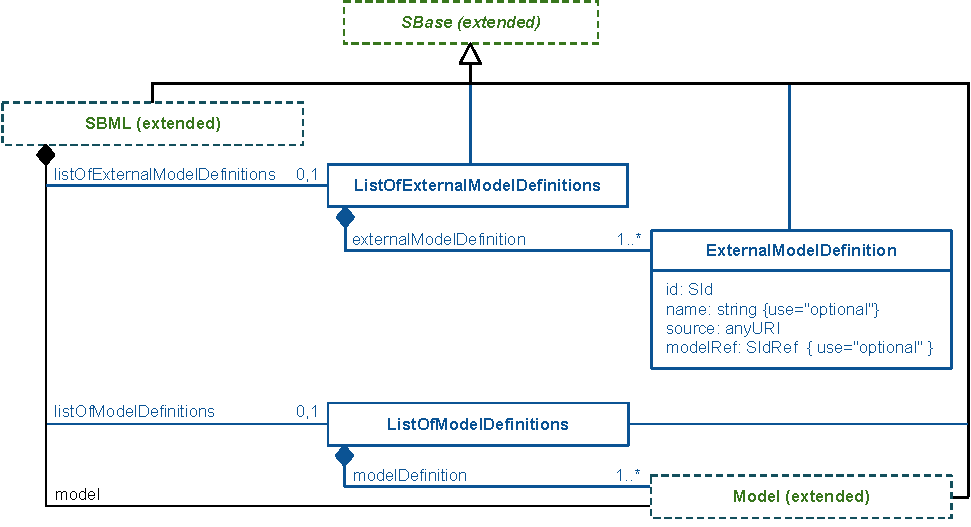
\includegraphics{figs/hierarchical-sbml}
  \caption{The definitions of the extended \SBML class as well as the
    new classes \ListOfModelDefinitions,
    \ListOfExternalModelDefinitions, and \ExternalModelDefinition.  The
    color conventions are explained in \protect\sect{conventions}.}
  \label{hierarchical-sbml-uml}
  \label{sbml-uml}
\end{figure}


\subsubsection{The lists of internal and external model definitions}

Model definition objects are not ``owned'' by any other model (they can
be instantiated anywhere, even by models in other files); therefore, the
approach used here pulls them out of the \Model class entirely, and
instead, puts them in a separate list.  The list is a child of the SBML
object itself.  Like other \textsf{\textbf{ListOf\rule{0.15in}{0.5pt}}}
classes in SBML, the \ListOfModelDefinitions is derived from \SBase
(more specifically, the extended \SBase class defined in
\sect{extenced-sbase-class}).  It inherits \SBase's attributes
\token{metaid} and \token{sboTerm}, as well as the subcomponents for
\Annotation and \Notes, but adds no especial attributes of its own.

If a model from an external SBML document is needed, it can be
referenced with an \ExternalModelDefinition object
(\sect{externalmodeldefinition-class}).  The
\ListOfExternalModelDefinitions container gathers all such references.
It is derived from \SBase but adds no especial attributes of its own.
Like the other \textsf{\textbf{ListOf\rule{0.15in}{0.5pt}}} classes, it
inherits the attributes \token{metaid} and \token{sboTerm}, as well as
the subcomponents for \Annotation and \Notes, that most SBML components
have.


\subsubsection{The \class{ExternalModelDefinition} class}
\label{externalmodeldefinition-class}

As mentioned above, references to externally-located models are
implemented as instances of \ExternalModelDefinition objects.  This
class is defined in \fig{hierarchical-sbml-uml}.  It contains several
attributes, two of them required (\token{source} and \token{id}), and
two of them optional (\token{modelRef} and \token{md5}).  These
attributes are defined in the subsections below.


\paragraph{The \hspace*{1pt}\token{id} attribute}

The \token{id} attribute serves to provide a handle for the external
model reference so that \Submodel objects can refer to it.  (Crucially,
it is \emph{not} the identifier of the model being referenced; rather,
it is an identifier for this \ExternalModelDefinition object within the
current model.)  The \token{id} attribute takes a required value of type
\primtype{SId}.


\paragraph{The \hspace*{1pt}\token{source} attribute}

The required attribute \token{source} is used to locate the SBML
document containing an external model definition.  The value of this
attribute must be of type \primtype{anyURI} (see \sect{primtype-uri}).
Since URIs may be either URLs, URNs, or relative or absolute file
locations, this offers flexibility in referencing SBML documents.  In
all cases, the \token{source} attribute value must refer specifically to
an SBML Level~3 Version~1 document; prior Levels/Versions of SBML are
not supported by this package.  The entire file at the given location is
referenced.  The \token{source} attribute must have a value for every
\ExternalModelDefinition instance.


\paragraph{The \hspace*{1pt}\token{modelRef} attribute}

\ExternalModelDefinition's optional attribute \token{modelRef}, of type
\primtype{SIdRef}, in is used to identify a \Model object within the
SBML document located at \token{source}.  The object referenced may be
the main model in the document, or a model definition contained in the
SBML document's \token{listOfModelDefinitions} list.

In standard SBML, \token{id} on \Model is an optional attribute, and
therefore, it is possible that the \Model object in a given SBML
document does \emph{not} have an identifier.  In that case, there is no
value to give to the \token{modelRef} attribute in
\ExternalModelDefinition.  If \token{modelRef} does \emph{not} have a
value, then the main model (i.e., the \token{<model>} element within the
\token{<sbml>} element) in the referenced file is interpreted as being
the model referenced by this \ExternalModelDefinition instance.


\paragraph{The \hspace*{1pt}\token{md5} attribute}

The optional \token{md5} attribute takes a \primtype{string} value.  If
set, it must be an MD5 checksum value computed over the document
referenced by \token{source}.  This checksum can be used as a data integrity
check over the contents of the \token{source}.  Applications may use
this to verify that the contents have not changed since the time that
the \ExternalModelDefinition reference was constructed.  The procedure
for using the \token{md5} attribute is described in
\tab{md5-procedures}.

\begin{table}[thb]
  \begin{edtable}{tabular}{p{1in}l@{\hspace{0.75ex}}p{5in}}
    \toprule
    \textbf{Case} & \multicolumn{2}{l}{\textbf{Procedure}} \\
    \midrule
    Creating and writing & 1.& Compute the MD5 hash for the document located at \token{source}.\\
    an SBML document     & 2.& Store the hash value as the value of the \token{md5} attribute. \\
    \midrule
    Reading an SBML      & 1.& Read the value of the \token{md5} attribute.\\
    document             & 2.& Read the document at the location indicated by the
                                \token{source} attribute value.\\
                         & 3.& Compute the MD5 hash for the document.\\
                         & 4.& Compare the computed MD5 value to the value in the \token{md5} attribute.  
                         If they are identical, assume the document has not changed since the
                         time the \ExternalModelDefinition object was defined; if the values
                         are different, assume that the document indicated by \token{source}
                         has changed. \\
    \bottomrule
  \end{edtable}
  \caption{Procedures for using the \token{md5} attribute on
    \ExternalModelDefinition.} 
  \label{md5-procedures}
\end{table}

Software tools encountering a difference in the MD5 checksums should
warn their users that a discrepancy exists, because a difference in the
documents may imply a difference in the mathematical interpretation of
the models.

Note that the MD5 approach is not without limitations.  An MD5 hash is
typically expressed as a 32-bit hexadecimal number.  If a difference
arises in the checksum values, there is no way to determine the cause of
the difference without an component-by-component comparison of the
models.  (Even a difference in annotations, which cannot affect a models' mathematical
interpretations, will result in a difference in the MD5 checksum
values.)  On the other hand, it is also not impossible that two
different documents yield the \emph{same} MD5 hash value, although it is
extremely unlikely in practice.  In any event, the MD5 approach is
intended as an optional, simple and fast data integrity check, and not a
final answer.


% -----------------------------------------------------------------------------
\subsection{The extended \class{Model} class}
\label{model-class}
\label{listofsubmodels-class}
\label{listofports-class}

In the Hierarchical Model Composition package, a model definition is, in
fact, a \Model object in a new context.  The SBML Level~3 Core \Model
class is extended here, and consists of two new lists: one for holding
submodels (\token{listOfSubmodels}, of class \ListOfSubmodels), and one
for holding a list of ports (\token{listOfPorts}, of class
\ListOfPorts).  The rest of this section defines the extended \Model
class and the \Port class, while the \Submodel class is described in
\sect{submodel-class}.

\begin{figure}[hbt]
  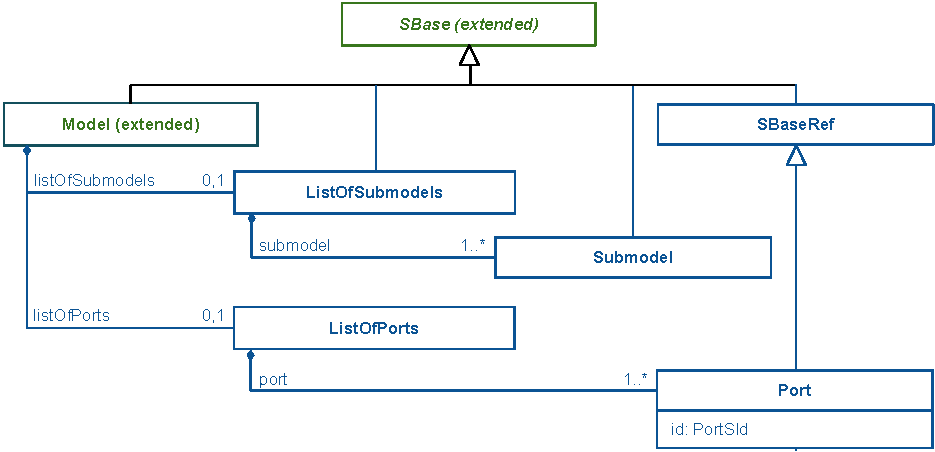
\includegraphics{figs/extended-model-uml}
  \caption{The extensions of the \Model class and the definitions of the
    classes \Port, \ListOfPorts, and \ListOfSubmodels.  \Submodel is
    defined in \sect{submodel-class}. In other respects, \Model remains
    defined as in the SBML Level~3 Core specification.}
  \label{extended-model-uml}
  \label{port-uml}
\end{figure}

Comparing the definition of \SBML in \fig{hierarchical-sbml-uml} with
the definition of \Model in \fig{extended-model-uml}, it becomes clear
that submodels are permitted both inside model definitions (the entities
contained by the \ListOfModelDefinitions) as well as in the top-level
model itself.  This is a key feature of the design that permits the
capabilities described in the introduction to the \sect{sbml-class}.
When the top-level model references submodels, they are instantiated,
whereas when the \Model object of a model definition references
submodels, they are simply part of that model definition---they are not
instantiated until the model definitions themselves are instantiated.


\subsubsection{The list of submodels}

The extended \Model class has an optional \token{listOfSubmodels}
subcomponent for holding a \ListOfSubmodels container object.  If
present, it must contain one or more \Submodel objects.  The \Submodel
class and its use is discussed separately in \sect{submodel-class}.


\subsubsection{The list of ports}

The \emph{port} concept allows a modeler to design a submodel such that
it can be used in a particular way by a containing model.  The intention
is that a modeler can indicate explicitly the intended points of
interaction between a (sub)model and other models including or otherwise
interacting with it.  Users of the model are encouraged to respect the
intention.  However, note that in the present formulation of the
Hierarchical Model Composition package, the use of ports is not
\emph{enforced}, nor is there any mechanism to place restrictions on
which ports may be used in what ways: they are only an advisory
construct.  Future versions of this package may incorporate these
attributes to provide additional functionality to support explicit
restrictions on port use.

In the Hierarchical Model Composition package, the concept of ports is
implemented in the the form of a \Port object and a list of ports
available on the extended \Model object (see \fig{extended-model-uml}).
Ports are elements that are designed to be used in replacements or
deletions, which are operations described below.


\subsubsection{The \class{Port} class}
\label{port-class}

The \Port class is defined in \fig{extended-model-uml}.  It is derived
from \SBaseRef, a class whose exact definition we leave to
\sect{sbaseref-class}; the class provides attributes \token{portRef},
\token{idRef}, \token{unitRef} and \token{metaIdRef}, and a recursive
subcomponent, \token{sbaseRef}.  In addition to what it inherits from
\SBaseRef, \Port adds one required attribute, \token{id}, described
below.

We say that a \Port object defines a port for a component in a model.
As will become clear in \sect{sbaseref-class}, the facilities of the
\SBaseRef parent class from which \Port is derived are what provides the
means for the component to be identified.  All of the options described
in \sect{sbaseref-class} for referencing other objects are available to
\Port objects.  For example, a port could be created by using the
\token{metaIdRef} attribute to identify the object for which a given
\Port instance is the port.  (In other words, ``what does this port
correspond to?'' is answered by the value of the \token{metaIdRef}
attribute.)


\paragraph{The \hspace*{1pt}\token{id} attribute}

The required attribute \token{id} is used to give an identifier to a
\Port object so that other objects can refer to it.  The attribute has
type \primtype{PortSId} and is essentially identical to the SBML
primitive type \primtype{SId}, except that its namespace is limited to
the identifiers of \Port objects defined within a \Model object.  In
parallel, the \primtype{PortSId} type has a companion type,
\primtype{PortSIdRef}, that corresponds to the SBML primitive type
\primtype{SIdRef}; the value space of \primtype{PortSIdRef} is limited
to \primtype{PortSId} values.  (See also \fig{sbaseref-uml}.)

Note the implication of the separate namespaces of port identifiers
(values of type \primtype{PortSId}) and other identifiers (values of
\primtype{SId} or \primtype{UnitSId}).  Since \primtype{PortSId} values
are in their own namespace within the parent \Model, it is possible for
a \primtype{PortSId} value to be the same as some \primtype{SId} value
in the model, without causing an identifier collision. 


\paragraph{Additional restrictions on \class{Port} objects}

Several additional restrictions exist on the use of ports.  It will
immediately become apparent that these restrictions are common-sense
rules, but they are worth making explicit:

\begin{enumerate}

  \item The model to which a \Port object refers with its \SBaseRef constructs
    must be the parent \Model object containing the \Port object itself.

  \item Each port in a model must refer to a unique component of that
    model; that is, no two ports in a model may both refer to the same
    model component.

  \item A port cannot refer to another port of the same model.

  \item A port cannot refer to itself.
    
\end{enumerate}
  
% \token{metaIdRef} attribute's value must refer to a meta identifier of
% an object in the immediately-enclosing \Model object.  (For example, it
% could refer to the \token{metaid} attribute value of a \Species object
% defined elsewhere in the model.)  This is a further restriction to the
% space of values than what is defined by XML \primtype{IDREF} alone.  The
% reason is simply that it makes no sense to allow one \Model object to
% define a port on a \emph{different} \Model object.  This does not imply
% a restriction or modification of the \token{metaid} values of \SBase
% objects in an SBML document, nor does it negate the other properties of
% XML type \primtype{IDREF}; it merely reduces the set of valid values
% that can be chosen for a given \token{metaIdRef} attribute on \Port
% objects in an SBML document.
%
% --See the new paragraph at the end of the SBaseRef section--it says (briefly) what it says in the above commented-out paragraph, but applies to all SBaseRef objects.


% -----------------------------------------------------------------------------
\subsection{The \class{Submodel} class}
\label{submodel-class}
\label{listofdeletions-class}

In the Hierarchical Model Composition package, submodels are the
concrete realization of models contained within other models.
\fig{submodel-uml} shows the definition of \Submodel.

\begin{figure}[hbt]
  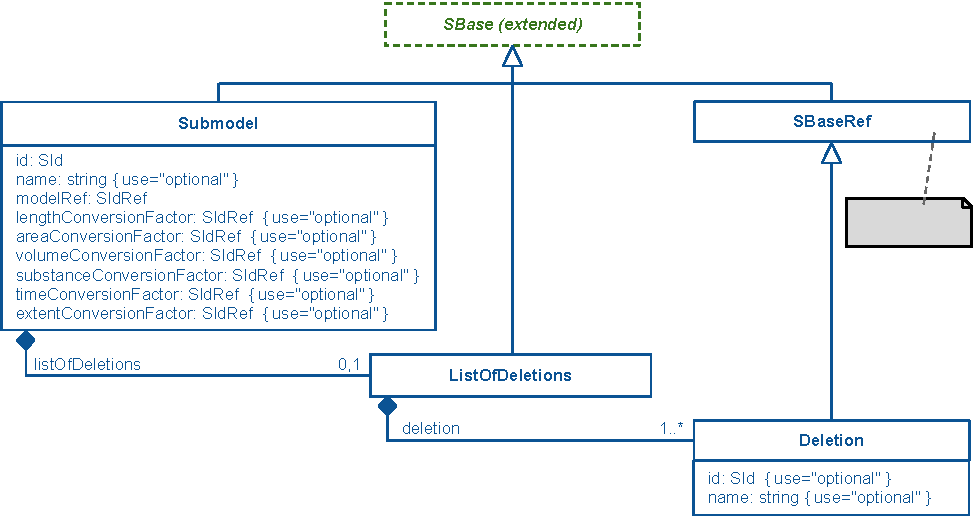
\includegraphics{figs/submodel-uml}
  \caption{The definition of the \Submodel, \Deletion and
    \ListOfDeletions classes.}
  \label{submodel-uml}
\end{figure}

A \Submodel object must say which \Model object it instantiates, and may
additionally contain information about how the \Model object is to be
modified.  There are two possible types of direct modifications:
conversion factors, and deletions.  We describe these two mechanisms in
more detail in the subsections below, but the following informal
description may serve as a useful guide.  If numerical values in the
referenced model must be changed in order to fit them into their new
context as part of the submodel, the changes can be handled through
conversion factors.  Deletions, on the other hand, are useful when a
feature in the referenced model no longer makes sense in its new context, have no equivalent in the new model,
and should be removed entirely; for example, it might be a
no-longer-relevant initial assignment, reaction, or an event assignment
within an \Event object.


\subsubsection{The attributes of \class{Submodel}}

\fig{submodel-uml} shows that \Submodel has numerous attributes, as well
as a single subcomponent, \token{listOfDeletions}.  We describe the
attributes below, then turn to \token{listOfDeletions} in
Sections~\ref{listofdeletions}--\ref{deletion-class}.


\paragraph{The \hspace*{1pt}\token{id} attribute}

The \token{id} is a required attribute of type \primtype{SId} that gives
an identifier to the \Submodel instance.  It is required so that other
references may always have a means through which a parent model may
refer to this submodel instance's elements (e.g., to link and replace
them).  The identifier has no mathematical meaning.

This identifier must follow the normal restrictions on SBML
\primtype{SId} values for uniqueness within \Model objects.  In
addition, the \token{id} value may not be referenced by SBML Level~3
Core components; this is necessary so that if a software package does
not have support for the Hierarchical Model Composition package, it can
ignore the package constructs and still end up with a syntactically
value (though perhaps diminished) SBML document.  


\paragraph{The \hspace*{1pt}\token{modelRef} attribute}
  
The \Model object that a \Submodel object instantiates may either be
another model in the same SBML document, or it may be a model defined in
a separate SBML document.  The required attribute \token{modelRef}, of
type \primtype{SIdRef}, must refer to the identifier of a \Model or
\ExternalModelDefinition object within the enclosing SBML document
(i.e., in the model namespace of the document).  

It is legal for the model referenced by \token{modelRef} to have its own submodels.
The chain of inclusion should be followed.  The only restriction is that
loops are not allowed: the referenced model may not refer to its parent
model, nor may it refer to a model which in turn instantiates its parent
model, etc.

It is also legal for the model referenced by \token{modelRef} to refer
to the \token{<model>} child of the enclosing SBML document, i.e., the
main \Model object in the \SBML object where it is itself located.  This
would mean that the document contains a model definition that itself
contains (and perhaps modifies) the model it presents to the world as
the main or top-level model in the document.  A possible use for this
might be to define a common scenario in the main model, then create
alternate scenarios with different initial conditions or parameter sets using the list of
model definitions (\fig{hierarchical-sbml-uml}) in the \SBML object.
Because the model namespace is defined per document, this means that it
is possible to define and include a new model namespace by creating a
new document, then importing one or more of those models using the
\ExternalModelDefinition class.


\paragraph{The conversion factor attributes}

Conversion factors enable the matching up of mathematical values and
units of measurement between submodels and models.  There are six
possible conversion factors, corresponding to the six conversion factors
defined by SBML Level~3 Core's basic \Model object class.  The six
attributes representing these conversion factors on \Submodel are
\token{lengthConversionFactor}, \token{areaConversionFactor},
\token{volumeConversionFactor}, \token{substanceConversionFactor},
\token{timeConversionFactor}, and \token{extentConversionFactor}.

All of these optional attributes have type \primtype{SIdRef}.  If set,
the value must be the identifier of a \Parameter object in the parent
\Model object.  The parameter will be used to convert the value of the
submodel quantities of the indicated type (e.g., volume, time, etc.) to
the units used in the parent model.  The procedures are involved, and a
separate section (\sect{conversion-factors}) is devoted to explaining
them.


\subsubsection{The list of deletions}
\label{listofdeletions}

The \token{listOfDeletions} subcomponent on \Submodel holds an optional
\ListOfDeletions container which, if present, must contain one or more
\Deletion objects.  This list of deletions specifies objects to be
removed from the submodel when composing the overall model.  (This
``removal'' of course does not involve physically editing the files;
rather, it is mathematical and conceptual.)

Deletions may be needed for various reasons.  For example, some
components in a submodel may be redundant in the composed model, perhaps
because the same features are implemented in a different way in the
new model.


\subsubsection{The \class{Deletion} class}
\label{deletion-class}

The \Deletion object class is used to define a deletion operation to be
applied when a submodel instantiates a model definition.  More
specifically, when the \Model to which the \Submodel object refers (via
the \token{modelRef} attribute) is read and processed for inclusion into
the composed model, each \Deletion object identifies an object to
``remove'' from that \Model instance.  The resulting submodel instance
will consist of everything in the \Model object instance minus the
entities referenced by the list of \Deletion objects.

As shown in \fig{submodel-uml}, \Deletion is subclassed from \SBaseRef,
described in detail in \sect{sbaseref-class}.  It reuses all the
machinery provided by \SBaseRef, and in addition, adds a single
attribute, \token{id}.


\paragraph{The \hspace*{1pt}\token{id} attribute}

The \Deletion attribute \token{id} can be used to give an identifier to
a given deletion.  The identifier has no mathematical meaning, but
providing it may be useful for creating submodels that can be
manipulated more directly by other submodels.


\paragraph{Implications of a deletion}

There are several points worth clarifying about deletions.

\begin{enumerate}

\item An object that has been ``deleted'' is considered inaccessible.
  Any element that has been replaced or deleted may not be referenced by
  an \SBaseRef object, including anything deleted or replaced within the
  submodel.

\item If the deleted object has child objects or substructure, the child
  objects and substructure are also considered to be deleted.

\item It is not an error to delete explicitly an object that is already
  deleted by implication (for example as a result of point number 2
  above).  The resulting model is the same.

\end{enumerate}

We leave additional comments about best practices surrounding deletions
to \sect{best-practices-deletions}.


% -----------------------------------------------------------------------------
\subsection{The \class{SBaseRef} class}
\label{sbaseref-class}

With the extensions to \SBML described up to this point, and the
introduction of \ExternalModelDefinition, the Hierarchical Model
Composition package constructs introduced so far have only provided a
means for aggregating models without \emph{connecting} them.  While this
may be useful for some applications, more interesting uses of
composition involving linking or restructuring components of different
models---for example, telling a simulator that some component \emph{X}
in one model is the same as a component \emph{Y} in a submodel, or
indicating that a given component \emph{Z} should be removed from the
composed whole model.  These operations require the capability to refer
to specific components within enclosed models or even external models
located in other files.  The machinery for constructing such references
is embodied in the \SBaseRef class.  This class is the parent class of
the \Port, \Deletion and \ReplacedElement classes described in the
previous sections.

\fig{sbaseref-uml} gives the definition of \SBaseRef.  It includes
several attributes used to implement alternative approaches to
referencing a particular component, and it also has a recursive
structure, providing the ability to refer to elements buried within
(say) a sub-submodel configuration.

\begin{figure}[hbt]
  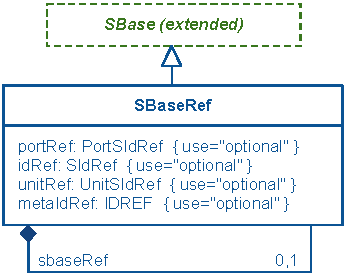
\includegraphics{figs/sbaseref-uml}
  \caption{The extensions of the \SBaseRef class.  The four attributes
    \token{portRef}, \token{idRef}, \token{unitRef} and \token{metaIdRef}
    are mutually exclusive; only one can have a value in a given object
    instance.  The recursive structure also allows referencing entities
    in submodels of submodels, to arbitrary depths, as described in the
    text.}
  \label{sbaseref-uml}
\end{figure}

Readers may wonder why so many different alternatives are necessary.
The reason is that in a given scenario, the referenced model may be
located in an external file beyond the direct control of the modeler,
and so the preferred methods of referencing the subobjects may not be
available.  \SBaseRef provides multiple alternatives so that a variety
of modeling scenarios can be supported.

%  far, we have described how to aggregate models together, and
% synchronize them so that their math is compatible.  A simulation of the
% resulting model would be equivalent to simulating the parent model and
% the submodels separately, scaling them appropriately, and then
% overlaying the results from each on the same graph.  This is usually not
% sufficient.  What is needed is a way to tell the simulator that this
% element of one submodel is the same as this other element of a second
% submodel.  In the case of a species, one submodel may control its
% creation and destruction, and the second may define how its presence
% modulates the rate of a related reaction.  It may have even been modeled
% as a constant parameter in the second submodel, if its concentration
% never changed under the conditions it was designed to imitate.  The new
% parent model may be an attempt to relax the assumptions in the
% submodels, and create a more complicated and robust model of the system
% being studied.


\subsubsection{The attributes of \class{SBaseRef}}

The four different attributes on \SBaseRef are mutually exclusive: only
one of the attributes can have a value at any given time, and exactly
one must have a value in a given \SBaseRef object instance.  (Note that
this is true of the basic \SBaseRef class; however, derived classes such
as \ReplacedElement may add additional attributes and extend or override
the basic attributes and mechanisms.)


\paragraph{The \hspace*{1pt}\token{portRef} attribute}

The optional attribute \token{portRef} takes a value of type
\primtype{PortSIdRef}.  As its name implies, this attribute is used to
refer to a port identifier, in the case when the reference being
constructed with the \SBaseRef is intended to refer to a port on a
submodel.  The namespace of the \primtype{PortSIdRef} value is the set
of identifiers of type \primtype{PortSId} defined in the submodel, not
the parent model.


\paragraph{The \hspace*{1pt}\token{idRef} attribute}

The optional attribute \token{idRef} takes a value of type
\primtype{SIdRef}.  As its name implies, this attribute is used to
refer to a regular identifier (i.e., the value of an \token{id}
attribute on some other object), in the case when the reference being
constructed with the \SBaseRef is intended to refer to an object that
does not have a port identifier.  The namespace of the \primtype{SIdRef}
value is the set of identifiers of type \primtype{SId} defined in the
submodel, not the parent model.


\paragraph{The \hspace*{1pt}\token{unitRef} attribute}

The optional attribute \token{unitRef} takes a value of type
\primtype{UnitSIdRef}.  This attribute is used to refer to the identifier
of a \UnitDefinition object.  The namespace of the \primtype{UnitSIdRef}
value is the set of unit identifiers defined in the submodel, not the
parent model.

Note that even though this attribute is of type \primtype{UnitSIdRef},
the reserved unit identifiers that are defined by SBML Level~3 (see
Section~3.1.10 of the SBML Level~3 Version~1 core specification) are
\emph{not} permitted as values of \token{unitRef}.  Reserved unit
identifiers may not be replaced or deleted.


\paragraph{The \hspace*{1pt}\token{metaIdRef} attribute}

The optional attribute \token{metaIdRef} takes a value of type XML
\primtype{IDREF}.  This attribute is used to refer to a \token{metaid}
attribute value on some other object, in the case when the reference
being constructed with the \SBaseRef is intended to refer to an object
that does not have a port identifier.  Since meta identifiers are
optional attributes of \SBase, all SBML objects have the potential to
have a meta identifier value.

\subsubsection{Recursive \class{SBaseRef} structures}

%% FIXME see LS's comments
%% Fixed (at least, I tried ;-) --LS

\SBaseRef has the capability to have up to one subcomponent of type
\SBaseRef named \token{sbaseRef} (see \fig{sbaseref-uml}), leading to
the possbility of constructing nested or recursive chains of references.
This feature can be used to refer to objects inside submodels in the
following way.  All parent \SBaseRef instances in the chain must refer to
a \Submodel (using either
\token{idRef}, \token{portRef} or \token{metaIdRef}, as suits the
particular object), and all child \SBaseRef objects in the chain must refer to an SBML component inside the \Model
instance to which the \Submodel refers.


\paragraph{Examples}

The following example may help clarify the nested structure.  Suppose
that we want to delete an object with the identifier \val{p1} inside the
\Submodel \val{m1}.  The following XML fragment illustrates how the
constructs will look:

\begin{example}
<listOfDeletions>
  <deletion idRef="m1">
    <sbaseRef idRef="p1" />
  </deletion>
</listOfDeletions>
\end{example}

If the desired element is within a submodel of a submodel (or deeper)
this nested construct can be extended to an arbitrary depth: as long as
an \SBaseRef object points to a \Submodel object, particular elements of
that submodel (including other submodels) may be referenced by a child
\SBaseRef.

% This is the original paragraph here --LS
%If instead, we had to make a reference to something contained inside a
%nested submodel within the submodel, then the child \SBaseRef object in
%\token{sbaseRef} will actually refer to the submodel's \Model or
%\ExternalModelDefinition instance, and it will have its own child
%\token{sbaseRef} object that then refers to a component inside the
%sub-submodel.  This can be repeated to accommodate arbitrary levels of
%submodel nesting.  

To illustrate that possibility, suppose that the submodel \val{m1} from
the previous example is actually nested inside another submodel
\val{m2}.  Then we would have the following:

\begin{example}
<listOfDeletions>
  <deletion idRef="m2">
    <sbaseRef idRef="m1">
      <sbaseRef idRef="p1" />
    </sbaseRef>
  </deletion>
</listOfDeletions>
\end{example}

Although this use of nested \SBaseRef objects allows a model to refer to
components buried inside submodels, it is considered inelegant model
design.  It is better to promote any element in a submodel to a local
element if it can be predicted that containing models may need to
reference it.  However, if the submodel is fixed (e.g., if is in an
external file), then no other option may be available except to use
nested references.

\subsubsection{Additional requirements for \class{SBaseRef}}

As mentioned in \sect{namespaces}, attributes of type \primtype{SId},
\primtype{UnitSId}, and \primtype{PortSId} need only be unique on a
per-\Model basis.  Therefore, a reader must also know the model to which
the \token{idRef}, \token{unitRef}, and \token{portRef} attributes
refer.  In addition, even though \primtype{IDREF} attributes are unique
on per-document level, the same SBML element may be instantiated in
multiple submodels, in any number of \Model objects, and therefore the
\token{metaIdRef} attribute must also know to which \Model instantiation
it is referring.  This will vary based on \SBaseRef sub-class, and will
be explained in those sections.  For ''bare'' \SBaseRef objects (which
only exist as children of other \SBaseRef objects, as explained above)
the \Model instance to which they are referring is the one referenced by
the \Submodel to which its parent is pointing.


% -----------------------------------------------------------------------------
\subsection{Replacements}
\label{replacements}
\label{extenced-sbase-class}

Replacements are the glue that connects submodels together with each
other and with the containing model.  To implement the replacement
mechanism, this package extends the SBML \SBase class as shown in
\fig{extended-sbase-uml}.

\begin{figure}[hbt]
  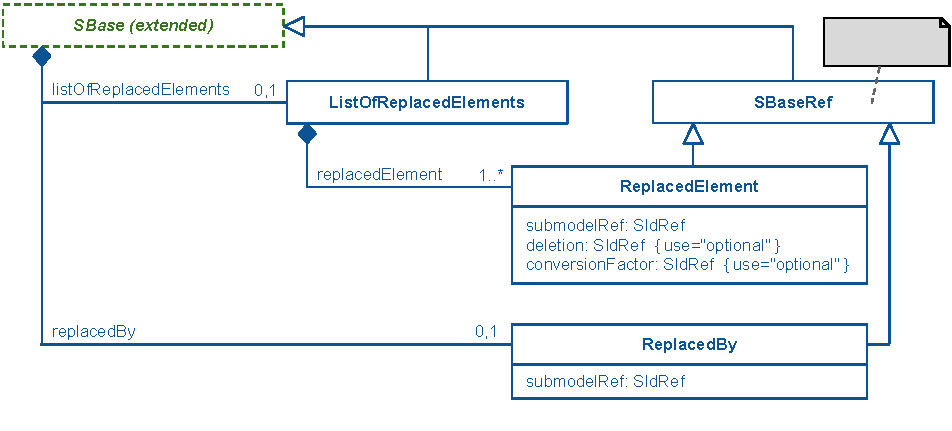
\includegraphics{figs/extended-sbase-uml}
  \caption{The extension of \SBase and the definition of the
    \ListOfReplacedElements and \ReplacedElement classes.  The \SBaseRef
  class is defined in \sect{sbaseref-class}.}
  \label{extended-sbase-uml}
\end{figure}


% Some previous proposal for model composition in SBML have called this
% concept 'links', as they link similar elements from different sources.
% All previous model composition proposals have lumped these things
% together in lists that were children of the Model class: one list of all
% replacements (or even all replacements and deletions) between this model
% and its submodels.

% Here, the concept of replacements is distributed to the individual
% elements that are replacing others.  This is accomplished by extending
% the \SBase class itself, as shown in \fig{extended-sbase-uml}.

\SBase in SBML is the abstract base class of almost all other object
classes.  It is not instantiated directly; rather, other SBML component
classes such as \Species, \Compartment and \Reaction objects are
subclassed from \SBase.  In this context, the list of replacements shown
in \fig{extended-sbase-uml} defines all of the replacements that
\emph{this} object (i.e., the concrete instantiation, be it a species,
parameter, or something else) replaces in any submodels where a
replacement is to be performed.  The nature of replacements will become
more clear in the \sect{replacedelement-class} below.


\subsubsection{The list of replaced elements}

\fig{extended-sbase-uml} shows that the extension of \SBase by the
Hierarchical Model Composition package adds an optional
\token{listOfReplacedElements} subcomponent for holding a
\ListOfReplacedElements container object.  If present, it must contain
at least one \ReplacedElement object.


\subsubsection{The \class{ReplacedElement} class}
\label{replacedelement-class}
\label{listofreplacedelements-class}

Replacements are a general mechanism that serve multiple purposes.  At
their most basic, they allow a model builder to make a statement of the
form ``entity \emph{W} in this model replaces entity \emph{X} in
submodel \emph{Y}''.  In the final composed model, all references to
\emph{X} in \emph{Y} are replaced with references to \emph{W}.  This
same approach is also used as the mechanism for linking or glueing
entities from different models together.  Thus, to establish a
connection between entity \emph{X} and some other entity \emph{Z}
located in another submodel, make \emph{W} define multiple replacements
simultaneously: one for \emph{X} and another for \emph{Z}.  Entity
\emph{W} acts as an intermediary at the level of the containing model.

The \ReplacedElement objects are essentially pointers to submodel
objects that are being replaced.  The object \emph{holding} the
\ReplacedElement instance is the one \emph{doing the replacing}; the
object pointed to by the \ReplacedElement object is the object being
replaced.  A replacement implies that the entire chain of dependencies
linked to the replaced object must be followed---all references to the
replaced object are instead taken to refer to the replacement object.
For example, if one species replaces another, then any reference to the
original species in mathematical formulas, or lists of reactants or
products or modifiers in reactions, or initial assignments, or any other
SBML construct, are taken to refer to the replacement species instead
(with its value possibly modified by either this object's
\token{conversionFactor} attribute or the relevant submodel's conversion
factors---see \sect{conversion-factors}).  Moreover, any annotations
that refer to the replaced species' \token{metaid} value must be made to
refer to the replacement species' \token{metaid} value instead; and
anything else that referred either to the object identifier (i.e., the
\token{id} attribute) or meta identifier (i.e., the \token{metaid}
attribute) must be made to refer to the replacement species object
instead.  

This identifier-redirection process has some additional important
implications.  First, when anything refers to a replaced object's
\token{id} and/or \token{metaid} value, the replacement object must
itself define its own \token{id} and/or \token{metaid} value, or else
the step of adjusting references will be impossible to perform because
there will not be new \token{id} or \token{metaid} values to use in
place of the old ones.  Second, if other SBML Level~3 packages attach
identifiers in their own namespaces to an object being replaced, those
identifiers must also be likewise redirected.  (And again, this implies
that the SBML document must put suitable identifier attributes from
those package namespaces on the \emph{replacement} object, so that the
replacement object's identifiers can be substituted for those of the
object being replaced.)

Finally, an important and far-reaching consequence of replacements is
that if the object being replaced contains other objects, then
\emph{those other objects are considered deleted}.  For example,
replacing a \Reaction or an \Event object means all of the substructure
of those entities in a model are deleted, and references to the
identifiers of those deleted entities are made invalid.


\paragraph{Attributes inherited from \class{SBaseRef}}

The \ReplacedElement class, being derived from \SBaseRef, inherits all
of that class' attributes and its subelement.  This means that
\ReplacedElement has the \token{portRef}, \token{idRef}, \token{unitRef}
and \token{metaIdRef} attributes, as well as the subcomponent
\token{sbaseRef} and the recursive structure that it implies.

It is the properties of \SBaseRef that allow a \ReplacedElement object
to refer to what is being replaced.  For example, if the object being
replaced has a \Port identifying it, the instance of \ReplacedElement would
have its \token{portRef} attribute value set to the id of the \Port pointing to 
the object being replaced.  If there is no corresponding \Port object, but
it has a regular identifier (typically an attribute named \token{id}), then
the \ReplacedElement object would set \token{idRef} instead, and so on.


\paragraph{The \hspace*{1pt}\token{submodelRef} attribute}
\label{replacedelement-submodelref}

The required attribute \token{submodelRef} takes a value of type
\primtype{SIdRef}.  It must be set to the identifier of a \Submodel
object in the containing model.  The \Model to which this \Submodel refers defines the object namespace to which the  \token{portRef}, \token{idRef}, \token{unitRef} and \token{metaIdRef} attributes refer.


\paragraph{The \hspace*{1pt}\token{identical} attribute}
\label{replacedelement-identical}

% FIXME:
%
% LS wrote: Also, I am now realizing that there's yet another caveat to the
% 'identical' attribute: not only can id's and metaid's be different in
% the replacement element, but any attribute that is an sidref, metaidref,
% or unitsidref may also be different.

The required attribute \token{identical} takes a \primtype{boolean}
value.  Its purpose is to indicate that a replacement is meant to be
effectively identical to the replaced object.  (This is the case when a
replacement only exists in order to create a reference to an object in a
submodel so that the containing model may work with that object.)

When \token{identical} has the value \val{true}, the two linked objects
are expected to be identical in all respects except possibly their
identifiers (i.e., their \token{id} and \token{metaid} attribute values,
as well as similar identifiers that may be added by other SBML Level~3
packages).  If the objects differ in any other way, validation systems
should report an error.  This applies to all attributes and
subcomponents, including \Annotation and \Notes subcomponents; even a
difference in the \token{name} attribute of the objects is considered a
deviation from being ``identical''.  Importantly, the numerical values
of all attributes (e.g., \token{initialAmount} on \Species) must be
equivalent to each other \emph{after accounting for any relevant
 conversion factors}.

When \token{identical} has the value \val{false}, no comparisons for
identical properties need to be performed, and no warnings or errors can
be reported if the two objects are or are not identical.


\paragraph{The \hspace*{1pt}\token{deletion} attribute}
\label{replacedelement-deletion}

The optional attribute \token{deletion} takes a value of type
\primtype{SIdRef}.  The value must be the identifier of a \Deletion object in
the parent \Model of the \ReplacedElement (that is, the value of some \Deletion object's \token{id}
attribute).  

When \token{deletion} is set, it means the \ReplacedElement object is
actually an annotation to indicate that the replacement object replaces
something deleted from a submodel.  The use of the \token{deletion}
attribute overrides the use of the attributes inherited from \SBaseRef:
instead of using, e.g., \token{portRef} or \token{idRef}, the
\ReplacedElement instance sets \token{deletion} to the identifier of the
\Deletion object.  The use of \ReplacedElement objects to refer to
deletions has no effect on the composition of models or the mathematical
properties of the result.  It serves instead to help record the
decision-making process that lead a modeler to construct the model they
did.  It can be particularly useful for visualization purposes, as well
as to serve as scaffolding where other types of annotations can be added
using the normal \Annotation subcomponents available on all \SBase
objects in SBML.

% Original text, some of which should go into the best practices:
%
% The most likely use case for this is in an 'N to M' replacement proposed
% by Andrew Finney ; perhaps an entire pathway is being replaced by a more
% detailed pathway with more reaction steps.  In this case, no one
% reaction step is replacing any one original reaction step, but the path
% as a whole is being conceptually replaced.  The way to implement this is
% to delete the original reaction steps from the submodel, and include the
% new reaction steps in the parent model.  If you wish to annotate those
% deletions, you may list the deletions as being replaced by elements of
% the new pathway.  This has no material effect on the model composition
% or on the math: it is merely a way to conceptually annotate the
% modeler's decision-making process.  As such, a deletion is the only type
% of Subelement that may be listed in more than one ListOfReplacements.
% It is recommended that in the above N to M scenario, all N deleted
% elements be listed under all M replacement elements, to make things
% easier on visualization software that may try to display the results.


\paragraph{The \hspace*{1pt}\token{conversionFactor} attribute}
\label{replacedelement-conversionfactor}

The \ReplacedElement's \token{conversionFactor} attribute may be used to
define how to transform or rescale the replaced object's value so that
it is appropriate for the new contexts in which it appears.  The value
of this attribute must be of type \primtype{SIdRef} and refer to a
\Parameter object instance defined in the model.  The conversion factor
identified by the \token{conversionFactor} attribute overrides any
automatic conversion that may have been performed based on the
submodel's relevant conversion factors.  The details of this are left to
\sect{conversion-factors}.


\paragraph{Additional requirements for \class{ReplacedElement}}
\label{replacedelement-additional}

The element in the parent model always takes precedence over elements
from the submodels, and no ``horizontal replacements'' are possible that
involve only subelements.  An example of horizontal replacement might be
when one species in one submodel is the conceptual replacement for a
second species in a second submodel.  In practice, the lack of a direct
mechanism for horizontal replacements is not a true limitation: to
achieve the same effect as in the example, a local species would be
created in the containing model replacing both species from the two
submodels, setting \token{identical}=\val{true} for the first, and
\token{identical}=\val{false} for the second.

% FIXME--is setting the \token like that the right thing to do, above? --LS DEBUG
% FIX: no, use the form \token{attributename}=\val{value}.

Note that there is no restriction here that replaced objects must be of
the same type as the replacing object.  The only restriction is that all
old references to the replaced object must now point to the replacing
object, so they must continue to make sense and produce valid SBML.
Thus, replacing a \Species object that appeared in a \Reaction object
would lead to an invalid SBML document if the replacement was a
\Parameter object.  There is no requirement for like-kind replacements,
however, because errors do not \emph{necessarily} result.  To take the
same example, the \Species object could be replaced by a \Parameter if
that \Species never appeared in any \Reaction object or if all the
\Reaction objects were deleted.  

Finally, any given object being replaced may only appear in exactly one
\ReplacedElement object anywhere in a model; otherwise, it would imply
multiple entities replace the same object, and this would lead to
ambiguities (e.g., in old references to the entities being replaced).  
A ``deletion'' \ReplacedElement (one that utilizes the 'deletion' attribute) is the sole exception to this rule, and
is the only type of entity that may be listed in more than one
\ListOfReplacedElements.


% -----------------------------------------------------------------------------
\subsection{Conversion factors}
\label{conversion-factors}

In SBML Level~3 Version~1 Core, units of measurement are optional
information.  Modelers are required to write their models in such a way
that all conversions between units are explicitly incorporated into the
quantities, so that nowhere do units need to be understood and values
implicitly converted before use.  Given the Hierarchical Model
Composition package's design goal of compatibility with existing models
and files that may not be changeable, it is not an option to require
that all included models must be written in such a way that they are
numerically compatible with each other.  For example, if one submodel
defines how a species amount changes in time, and a second submodel
defines an initial assignment for that same species in terms of
concentration, something must be done to make the model as a whole
coherent without editing the submodels directly.  That is the purpose of
the conversion factor attributes on the \Submodel and \ReplacedElement
classes.

There are many situations to account for, so unfortunately, the topic of
conversion factors is rather involved.  We begin with the relatively
straightforward case of \ReplacedElement.


\subsubsection{Conversion factors involving \class{ReplacedElement}}

As explained in \sect{replacedelement-class}, the various conversion
factor attributes on \ReplacedElement override any conversion factors
defined on the \Submodel object that the \ReplacedElement references via
its \token{modelRef} attribute.

If the submodels of the merged model retain any mathematical formulas
(that is, if there are any reactions, assignments, or any other
construct with a MathML \token{<math>} element that has not been
replaced or deleted from the submodel), then those formulas may be
subject to different scales and units than the mathematical formulas of
the containing model.  In that case, the entities and formulas should be
converted to the new units.  If a replaced element has a defined
conversion factor, then any time a calculation is performed within the
math of the \Submodel object where the replaced element's identifier is
found on the left-hand side of an equation, the right-hand side is
multiplied by that conversion factor before assignment to that variable.
For example, if a species has an initial assignment of $4x + 3$, and has
a conversion factor of $c$, the initial assignment formula become
$c (4x+3)$.  The same is true for assignment rules, rate
rules, kinetic laws, event assignments, and the implied rates of change
of species as calculated from kinetic laws, as described in section
4.11.7 of the SBML Level~3 Version~1 Core specification.

Conversely, wherever the identifier of a replaced element appears on the
right-hand side of an equation in its original submodel, its appearance
in that equation should be \emph{divided} by the conversion factor.  In
our previous example of an initial assignment of $4x+3$, if the $x$ had
been replaced and given a conversion factor of $c_x$, that initial
assignment formula would become $4(x/c_x)+3$.  This holds true for any
mathematical equation in the model, including algebraic rules.  This
also means that if a value appears on the right and left-hand sides of
an equation, you must apply the conversion factor twice: if the rate
rule of $x$ is $4x+3$, it becomes $c_x(4(x/c_x) + 3)$.  (This
simplifies to $4x + 3c_x$, as you would expect---the $x$ is already in
the correct scale; it is only the 3 that must be converted.)

% The situation becomes trickier when talking about implied units of model
% elements.  The SBML Level~2 specification defined what the 'base units'
% of the model were, even if none were defined in the model itself.  SBML
% Level 3 no longer does this, but it retains the concept of unit types
% for certain elements, even if those units are left undefined.  A
% compartment with 'spatialDimensions=3' is of the unit type 'volume', for
% example, even if exactly what units those are (liters; millicubits3;
% etc.) is left undefined.  Similarly, all species are either of the unit
% type 'substance' or 'concentration', depending on the value of the
% required Boolean attribute 'hasOnlySubstanceUnits'.  ('Concentration'
% is, in turn, defined as 'substance divided by the units of the
% containing compartment'.)  Rate rules of elements are defined as the
% unit of that element divided by time.  The implied equations derived
% from reactions (see section 4.11.7 of the core specification) are
% defined as being substance over time.  Regardless of what those units
% are defined to be, or even if those units are left undefined, the unit
% types are set, and must be consistent throughout the model, so nothing
% is implicitly converted.


\subsubsection{Conversion factors involving \class{Submodel}}

The six attributes on \Submodel with the names of the form
\token{\rule{0.2in}{0.5pt}ConversionFactor} dictate how any submodel
mathematics whose unit types are defined by the Level~3 Core
specification are to be converted whether or not that element was
replaced, in the absence of an explicit conversion factor for that
element.  To understand the rules, it is first helpful to have a summary
of the conversion factors implied by the SBML Level~3 Version~1 Core
specification.  We provide a summary in \tab{sbml-conversions}.

\newcommand{\sprd}[2]{\raisebox{-#1pt}[0pt][(#1pt * 2) + 4pt]{#2}}
\newcommand{\persymb}{\emph{Conversion factor for referenced object}}
\newcommand{\percomp}{\emph{Conversion factor for compartment}}
\newcommand{\allat}{\emph{(All)}}
\newcommand{\hosu}{\token{hasOnlySubstanceUnits}}

\begin{table}[bht]
  \rowcolors{2}{sbmlrowgray}{}
  \renewcommand{\arraystretch}{1.175}
  \begin{edtable}{tabular}{p{1.1in}p{2.57in}l}
    \toprule
    \textbf{Component}	& \textbf{Attribute value}	& \textbf{Automatic conversion factor}\\
    \midrule
    \AlgebraicRule	& \allat			& 1\\
    \AssignmentRule	& \allat			& \persymb\\
    \Compartment	& \token{spatialDimensions}=\val{1}	& \token{lengthConversionFactor}\\
    \Compartment	& \token{spatialDimensions}=\val{2}	& \token{areaConversionFactor}\\
    \Compartment	& \token{spatialDimensions}=\val{3}	& \token{volumeConversionFactor}\\
    \Compartment	& \token{spatialDimensions} not equal to \val{1}, \val{2}, or \val{3} & 1\\
    \Constraint		& \allat			& \emph{(None needed)}\\
    \Delay		& \allat			& \token{timeConversionFactor}\\
    \EventAssignment	& \allat			& \persymb\\
    \FunctionDefinition	& \allat			& 1\\
    \InitialAssignment	& \allat			& \persymb\\
    \sprd{4}{\KineticLaw} & \sprd{4}{\allat}		& \sprd{4}{$\frac{\token{extentConversionFactor}}{\token{timeConversionFactor}}$}\\
    Implied rate of change of a species	& \sprd{4}{\allat}		& \sprd{4}{$\frac{\token{substanceConversionFactor}}{\token{timeConversionFactor}}$}\\
    \Parameter		& \allat			& 1\\
    \Priority		& \allat			& 1\\
    \sprd{4}{\RateRule} & \sprd{4}{\allat}		& \sprd{4}{$\frac{\textsf{\persymb}}{\token{timeConversionFactor}}$}\\
    \Species		& \hosu=\val{true}		& \token{substanceConversionFactor}\\
    \sprd{4}{\Species}	& \sprd{4}{\hosu=\val{false}}	& \sprd{4}{$\frac{\token{substanceConversionFactor}}{\textsf{\persymb}}$}\\
    \sprd{6}{\Species}	& \hosu=\val{true} replaced by a \Species having \hosu=\val{false}
	    & \sprd{6}{$\frac{\token{substanceConversionFactor}}{\textsf{\emph{Compartment size}}}$}\\
    \sprd{6}{\Species}	& \hosu=\val{false} replaced by a \Species having \hosu=\val{true}
	    & \sprd{6}{$\frac{\token{substanceConversionFactor} \,\cdot\, \textsf{\emph{(Compart. size)}}}{\percomp}$}\\
    \SpeciesReference	& \allat			& 1\\
    \Trigger		& \allat			& \emph{(None needed)}\\
    (Unknown)		& \allat			& 1\\
    \bottomrule
  \end{edtable}
  \caption{Conversion factors used for the different components defined
    by SBML Level~3 Core.}
  \label{sbml-conversions}
\end{table}

The procedures for using the conversion factor attributes on \Submodel
are based on the conversion factors defined by the Core.  Thus, all
compartments that set \token{spatialDimension}=\val{1} in the submodel
must be converted according to the \token{lengthConversionFactor}, with
all assignments to that compartment multiplied by the conversion factor,
and that compartment's identifier divided by it wherever it appears
inside a math element.  All rates of change of species amounts (defined
in section 4.11.7 of the Level~3 Version~1 Core specification) are
converted by the \token{substanceConversionFactor} divided by the
\token{timeConversionFactor}, after being converted (if necessary) by
any internal conversion factors, as described.  All species
concentrations from compartments of dimension 2 are converted by the
\token{substanceConversionFactor} divided by the
\token{areaConversionFactor}.  Non-replaced elements with defined unit
types are still converted, so that the output of any simulation will be
on the same scale as elements from the containing model.

In the core specification for SBML Level 3, if the conversion factor
attributes for \Model and \Species are undefined, the rate of change of
species amounts over time is defined to be equal to the rate of extent
of the reaction over time, arguably creating a default conversion of
extent to amount of 1.  Similarly, all conversion factors here
effectively default to '1' as well, so that if (for example)
'substanceConversionFactor' is defined but 'areaConversionFactor' is
not, species concentrations from compartments of dimension 2 are still
converted according to the substanceConversionFactor, 'divided by 1'.

Critically, if an element's unit type cannot be determined, it has no
default conversion factor, and one must be set explicitly for the
element in question.  All \Parameter objects fall into this category, as
parameters may have any unit at all, and have no defined unit type as a
class.  Similarly, compartments with no \token{spatialDimension} set, or
set to a fractal \token{spatialDimension} such as 2.6 should not be
converted automatically.  This means that if a parameter is internal to
a submodel and not replaced, there is no way to convert it, and it will
remain in its original scale.  This will not affect the math of the
converted elements, as the rules above first convert all math to the
original scale, and only convert it to the new scale when assigning it
to a variable.  However, if it is displayed as output, these values may
be in a different scale from other displayed output.  The only way to
correct this situation is to replace the parameter in question, and give
it an explicit conversion factor.

Some math may use a combination of conversion factors defined on the
\Submodel object with the conversion factors defined explicitly on an
element's replacement construct.  The simplest example is that of a rate
rule that defines how a parameter changes with time.  If the \Parameter
object has been replaced and given a conversion factor, the parameter's
explicit conversion factor is divided by the submodel's
\token{timeConversionFactor} to act as the overall conversion factor for
the rate rule's formula.  As a slightly more complicated example, a
species concentration that has no explicit conversion factor set for its
replacement, and which is contained in a compartment that does have an
explicit conversion factor, will be converted according to the
\token{substanceConversionFactor} from the \Submodel object divided by
the conversion factor defined by the compartment replacement construct.

Species concentrations of species from compartments with undefined unit
types will be converted according to the
\token{substanceConversionFactor} alone, if no conversion factor is
defined for its compartment.  An odd potential situation arises here in
the case where the species' compartment has been actually deleted
instead of replaced, the replacement species being put into a new
compartment in the containing model.  In this case, no automatic
conversion factor is possible, and if one is needed, it must be set
explicitly on the species' replacement itself.  Another complication is
the situation where a species is set
\token{hasOnlySubstanceUnits}=\val{true} in the submodel, but is set
\token{hasOnlySubstanceUnits}=\val{false} in its replacement, or vice
versa.  In this case, the species must be converted according to the
actual value of its compartment.  If an explicit conversion factor is
set, it is assumed that the modeler took this into consideration, and
created an assignment rule (or similar) such that the conversion
parameter would function appropriately.  If not, the automatic
conversion must use the value for the compartment of the replacement
species to convert the species values to amounts from concentrations,
and back again.  Unreplaced species are still converted, but if they
were in amounts before, they remain in amounts afterwards and likewise
when in concentrations.

Any math not directly associated with a replaced element and that does
not have a defined unit type is assumed to exist in the same scale as
all other similar elements across all submodels.  The only example of
this in the Level~3 Core is the math associated with the \Priority
subcomponent of \Event objects.  A \Priority element may be replaced
directly by a \ReplacedElement construct or by replacing its parent
\Event, but when comparing priority expressions from submodels with
priority expressions from the containing model or from other submodels,
they are all assumed to be on the same scale relative to each other.
(If one model had priorities set on a scale of 0 to 10 and another had
priorities set on a scale of -100 to 100, that is just the way it is,
and to fix it, all incompatible priorities would have to be replaced.)
The same would be true of math defined in any other Level~3 package
without a defined unit type, or with a newly-defined unit type: none of
it would be converted automatically, and all such elements would have to
be converted explicitly by being replaced, or that package would have to
extend this Hierarchical Model Composition package to define a new
attribute on Submodel that could be used to automatically convert all
such elements in the submodel with that unit type.

